%& -shell-escape
\title{Linear Regression}
\author{Ahnaf An Nafee}
\date{February 2021}
\documentclass[12pt]{article}
\usepackage[margin=0.7in]{geometry}
\usepackage{graphicx}
\usepackage{float}
\usepackage{amsmath}
\usepackage{multicol}
\usepackage{comment}
\usepackage{listings}
\usepackage{xcolor}
\usepackage{multirow}

\graphicspath{ {./images/} }

\definecolor{codegreen}{rgb}{0,0.6,0}
\definecolor{codegray}{rgb}{0.5,0.5,0.5}
\definecolor{codepurple}{rgb}{0.58,0,0.82}
\definecolor{backcolour}{rgb}{0.95,0.95,0.92}

\lstdefinestyle{mystyle}{
	backgroundcolor=\color{white},   
	commentstyle=\color{codegreen},
	keywordstyle=\color{magenta},
	numberstyle=\tiny\color{codegray},
	stringstyle=\color{codepurple},
	basicstyle=\ttfamily\footnotesize,
	breakatwhitespace=false,         
	breaklines=true,                 
	captionpos=b,                    
	keepspaces=true,                 
	numbers=left,                    
	numbersep=5pt,                  
	showspaces=false,                
	showstringspaces=false,
	showtabs=false,                  
	tabsize=2
}

\lstset{style=mystyle}


\begin{document}

\maketitle

\section{Theory}

\begin{enumerate}
	\item LR Supervised Training Dataset:


\begin{enumerate}
	
	\item Coefficients for Closed-form Linear Regression:\\

		$
		X=
		\begin{bmatrix}
			1 & -2\\
			1 & -5\\	
			1 & -3\\
			1 & 0\\
			1 & -8\\
			1 & -2\\
			1 & 1\\
			1 & 5\\
			1 & -1\\
			1 & 6\\
		\end{bmatrix},
	Y=
		\begin{bmatrix}
			1\\
			-4\\	
			1\\
			3\\
			11\\
			5\\
			0\\
			-1\\
			-3\\
			1\\
		\end{bmatrix}
		$



	\begin{equation}
		\begin{split}
			w = \frac{1}{N} (X^{T}X)^{-1}X^{T}Y
		\end{split}
	\end{equation}

	\begin{equation}
	\begin{split}
		w = (\begin{bmatrix}
			1 & -2\\
			1 & -5\\	
			1 & -3\\
			1 & 0\\
			1 & -8\\
			1 & -2\\
			1 & 1\\
			1 & 5\\
			1 & -1\\
			1 & 6\\
		\end{bmatrix}^{T}\begin{bmatrix}
			1 & -2\\
			1 & -5\\	
			1 & -3\\
			1 & 0\\
			1 & -8\\
			1 & -2\\
			1 & 1\\
			1 & 5\\
			1 & -1\\
			1 & 6\\
		\end{bmatrix})^{-1}\begin{bmatrix}
			1 & -2\\
			1 & -5\\	
			1 & -3\\
			1 & 0\\
			1 & -8\\
			1 & -2\\
			1 & 1\\
			1 & 5\\
			1 & -1\\
			1 & 6\\
		\end{bmatrix}^{T}\begin{bmatrix}
			1\\
			-4\\	
			1\\
			3\\
			11\\
			5\\
			0\\
			-1\\
			-3\\
			1\\
			\end{bmatrix}
		\end{split}
	\end{equation}

\begin{equation}
	\begin{split}
		w = (\begin{bmatrix}
			1 & 1 & 1 & 1 & 1 & 1 & 1 & 1 & 1 & 1\\
			-2 & -5 & -3 & 0 & -8 & -2 & 1 & 5 & -1 & 6\\
		\end{bmatrix}\begin{bmatrix}
			1 & -2\\
			1 & -5\\	
			1 & -3\\
			1 & 0\\
			1 & -8\\
			1 & -2\\
			1 & 1\\
			1 & 5\\
			1 & -1\\
			1 & 6\\
		\end{bmatrix})^{-1}\begin{bmatrix}
		1 & -2\\
		1 & -5\\	
		1 & -3\\
		1 & 0\\
		1 & -8\\
		1 & -2\\
		1 & 1\\
		1 & 5\\
		1 & -1\\
		1 & 6\\
	\end{bmatrix}^{T}\begin{bmatrix}
			1\\
			-4\\	
			1\\
			3\\
			11\\
			5\\
			0\\
			-1\\
			-3\\
			1\\
		\end{bmatrix}
	\end{split}
\end{equation}

\begin{equation}
	\begin{split}
		w = (\begin{bmatrix}
			10 & -9\\
			-9 & 169\\
		\end{bmatrix})^{-1}\begin{bmatrix}
		1 & 1 & 1 & 1 & 1 & 1 & 1 & 1 & 1 & 1\\
		-2 & -5 & -3 & 0 & -8 & -2 & 1 & 5 & -1 & 6\\
	\end{bmatrix}\begin{bmatrix}
			1\\
			-4\\	
			1\\
			3\\
			11\\
			5\\
			0\\
			-1\\
			-3\\
			1\\
		\end{bmatrix}
	\end{split}
\end{equation}

\begin{equation}
	\begin{split}
		w = (\begin{bmatrix}
			0.10503418 & 0.00559354\\
			0.00559354 & 0.00621504\\
		\end{bmatrix})\begin{bmatrix}
			1 & 1 & 1 & 1 & 1 & 1 & 1 & 1 & 1 & 1\\
			-2 & -5 & -3 & 0 & -8 & -2 & 1 & 5 & -1 & 6\\
		\end{bmatrix}\begin{bmatrix}
			1\\
			-4\\	
			1\\
			3\\
			11\\
			5\\
			0\\
			-1\\
			-3\\
			1\\
		\end{bmatrix}
	\end{split}
\end{equation}

\begin{equation}
	\begin{split}
		w = \begin{bmatrix}
			0.10503418 & 0.00559354\\
			0.00559354 & 0.00621504\\
		\end{bmatrix}\begin{bmatrix}
			14\\
			-79\\
		\end{bmatrix}
	\end{split}
\end{equation}

\begin{equation}
	\begin{split}
		w = \begin{bmatrix}
			1.02858919\\
			-0.41267868\\
		\end{bmatrix}
	\end{split}
\end{equation}



		\begin{comment}
	\newpage
	\end{comment}
	
	\newpage
	
	\item Predictions, Y , for the Training Data:\\
	
	$
		Y_{pred}=
	\begin{bmatrix}
		1.8539465\\
		3.0919826\\	
		2.2666252\\
		1.0285892\\
		4.3300186\\
		1.8539466\\
		0.6159105\\
		-1.0348042\\
		1.4412679\\
		-1.4474829\\
	\end{bmatrix}
	$


	\item RMSE:\\
	
		\begin{lstlisting}[language=Python]
			def rmse(predictions, targets):
				return np.sqrt(np.mean((predictions-targets)**2))
				
			print("RMSE: ", rmse(Ypred, Y))
		\end{lstlisting}
	
	\textbf{RMSE}: $3.701325917666$

		
	
	\end{enumerate}
	
	\begin{comment}
	\newpage
		\end{comment}


	\item Function Weights:\\
	
	\begin{enumerate}
	
	\item Partial Gradients:\\
	
	$J=(x_1 w_1 -5x_2 w_2-2)^2$ = $(x_1 w_1 -5x_2 w_2-2)$$(x_1 w_1 -5x_2 w_2-2)$\\
	$J=x_1^{2}w_1^{2} - 5x_{1}x_{2}w_{1}w_{2}-2x_{1}w_{1}-5x_{1}x_{2}w_{1}w_{2} + 25x_2^{2}w_2^{2} + 10x_{2}w_2-2x_{1}w_{1} +10x_{2}w_{2} + 4$\\
	$J=x_1^{2}w_1^{2} - 10x_{1}x_{2}w_{1}w_{2} -4x_{1}w_{1} + 25x_2^{2}w_2^{2} + 20x_{2}w_{2} + 4$\\
	
	
	\begin{equation}
		\begin{split}
			\frac{\partial J}{\partial w_1} = 2x_1^{2}w_1 - 10x_{1}x_{2}w_{2} - 4x_{1}
		\end{split}
	\end{equation}

	\begin{equation}
		\begin{split}
			\frac{\partial J}{\partial w_2} = -10x_{1}x_{2}w_{1} + 50x_2^{2}w_2 + 20x_2
		\end{split}
	\end{equation}
	
	\item Value of the Partial Gradients:\\
	
	\begin{tabular}{ c c}
		$w_1 = 0$ & $x_1 = 1$\\ 
		$w_2 = 0$ & $x_2 = 1$ 
	\end{tabular}\\
\\
	
	$\frac{\partial J}{\partial w_1} = 2 \times 0^2 \times 1 - 10 \times 1 \times 1 \times 0 - 4 \times 1 = -4$\\
	$\frac{\partial J}{\partial w_2} = - 10 \times 1 \times 1 \times 0 + 50 \times 1^2 \times 0 + 20 \times 1 = 20$\\
	

	\end{enumerate}

	
	\begin{comment}

	\end{comment}
	

\end{enumerate}

\newpage

\section{Gradient Descent}

	\begin{enumerate}
		
		\item Plot of epoch vs $J$:\\
		
		\begin{center}
			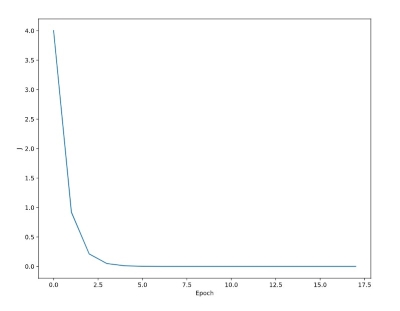
\includegraphics{epoch_vs_J}
		\end{center}
		
		\item 3D plot of $w_1$ vs $w_2$, vs $J$:\\
		
		\begin{center}
			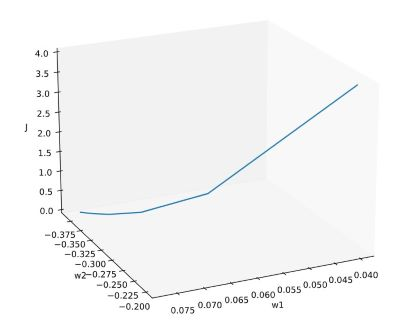
\includegraphics{w1_vs_w2_vs_J}
		\end{center}
		
		\newpage
		
		\item Final learned values of $w_1$, $w_2$, and $J$, and the number of epochs required to get there:\\
		
		Converged at Epoch:  $18$\\\\
		$w_1 = 0.07692293618911292$\\ 
		$w_2 = -0.3846146809455646$\\
		$J = 5.8111496830407836^{-11}$
		
	\end{enumerate}
	


\section{Closed Form Linear Regression}

	\begin{enumerate}
		

		\item 
		RMSE (TRAINING - ENUM - NO BIAS):  $\textbf{151357.23969016664}$\\
		RMSE (TESTING - ENUM - NO BIAS):  $\textbf{181121.86523476854}$\\
		
		\item
		RMSE (TRAINING - ENUM - BIAS):  $\textbf{5757.954440690525}$\\
		RMSE (TESTING - ENUM - BIAS):  $\textbf{6519.373997851638}$\\
		
		\item
		RMSE (TRAINING - BIN - NO BIAS):  $\textbf{31707.42718070179}$\\
		RMSE (TESTING - BIN - NO BIAS):  $\textbf{31434.144622561682}$\\
		
		\item
		RMSE (TRAINING - BIN - BIAS):  $\textbf{5763.9397804300825}$\\
		RMSE (TESTING - BIN - BIAS):  $\textbf{6502.067257403235}$\\


	\end{enumerate}

\end{document}
